%%%%%%%%%%%%%%%%%%%%%%%%%%%%%%%%%%%%%%%%%
% Beamer Presentation
% LaTeX Template
% Version 1.0 (10/11/12)
%
% This template has been downloaded from:
% http://www.LaTeXTemplates.com
%
% License:
% CC BY-NC-SA 3.0 (http://creativecommons.org/licenses/by-nc-sa/3.0/)
%
%%%%%%%%%%%%%%%%%%%%%%%%%%%%%%%%%%%%%%%%%

%----------------------------------------------------------------------------------------
%	PACKAGES AND THEMES
%----------------------------------------------------------------------------------------

\documentclass{beamer}

\mode<presentation> {

% The Beamer class comes with a number of default slide themes
% which change the colors and layouts of slides. Below this is a list
% of all the themes, uncomment each in turn to see what they look like.

%\usetheme{default}
%\usetheme{AnnArbor}
%\usetheme{Antibes}
%\usetheme{Bergen}
%\usetheme{Berkeley}
%\usetheme{Berlin}
%\usetheme{Boadilla}
%\usetheme{CambridgeUS}
%\usetheme{Copenhagen}
%\usetheme{Darmstadt}
%\usetheme{Dresden}
%\usetheme{Frankfurt}
%\usetheme{Goettingen}
%\usetheme{Hannover}
%\usetheme{Ilmenau}
%\usetheme{JuanLesPins}
%\usetheme{Luebeck}
\usetheme{Madrid}
%\usetheme{Malmoe}
%\usetheme{Marburg}
%\usetheme{Montpellier}
%\usetheme{PaloAlto}
%\usetheme{Pittsburgh}
%\usetheme{Rochester}
%\usetheme{Singapore}
%\usetheme{Szeged}
%\usetheme{Warsaw}

% As well as themes, the Beamer class has a number of color themes
% for any slide theme. Uncomment each of these in turn to see how it
% changes the colors of your current slide theme.

%\usecolortheme{albatross}
%\usecolortheme{beaver}
%\usecolortheme{beetle}
%\usecolortheme{crane}
%\usecolortheme{dolphin}
%\usecolortheme{dove}
%\usecolortheme{fly}
%\usecolortheme{lily}
%\usecolortheme{orchid}
%\usecolortheme{rose}
%\usecolortheme{seagull}
%\usecolortheme{seahorse}
%\usecolortheme{whale}
%\usecolortheme{wolverine}

%\setbeamertemplate{footline} % To remove the footer line in all slides uncomment this line
\setbeamertemplate{footline}[page number] % To replace the footer line in all slides with a simple slide count uncomment this line

\setbeamertemplate{navigation symbols}{} % To remove the navigation symbols from the bottom of all slides uncomment this line
%\setbeamercovered{transparent} % to show what is coming in the next slide
}

\usepackage{graphicx} % Allows including images
\usepackage{booktabs} % Allows the use of \toprule, \midrule and \bottomrule in tables
\usepackage{amsmath, amsthm, amscd, amsfonts, amssymb, graphicx, color}
\usepackage{mathtools,textcomp}
\usepackage[latin1]{inputenc}
\usepackage{amsmath,amssymb}

\usepackage{subcaption}
\usepackage{multirow}
\usepackage{caption}
\usepackage{tikz, tcolorbox}

\newcommand{\bm}{\boldsymbol}
\newcommand\emachine{\epsilon_{\text{machine}}}
\newcommand\bH{\bm H}
\newcommand\bI{\bm I}
\newcommand\bF{\bm F}
\newcommand\bU{\bm U}
\newcommand\bN{\bm N}
\newcommand\bv{\bm v}
\newcommand\bn{\bm n}
\newcommand\bR{\bm R}
\newcommand\bS{\bm S}
\newcommand\btau{\bm \tau}
\newcommand\bC{\bm C}
\newcommand\bb{\bm b}
\newcommand\bE{\bm E}
\newcommand\be{\bm e}
\newcommand\bx{\bm x}
\newcommand\bX{\bm X}
\newcommand\bu{\bm u}
\newcommand\bulk{k}
\newcommand\firstlame{\mathsf{\lambda}}
\newcommand\tcolon{\!:\!}
\newcommand\trace{\operatorname{trace}}
\newcommand\diff{\operatorname{d}\!}
\newcommand\Det[1]{\lvert #1 \rvert}
\newcommand\sign{\operatorname{sign}}
\newcommand\fl{\operatorname{fl}}
\newcommand\expm{\operatorname{\mathtt{expm1}}}
\newcommand\logp{\operatorname{\mathtt{log1p}}}
\newcommand\logpmx{\operatorname{\mathtt{log1p\_minus\_x}}}
\newcommand\Jm{\mathtt{J_{-1}}}
\newcommand{\dd}[2]{\frac{\partial #1}{\partial #2}}
\newcommand{\code}[1]{\textsf{#1}}
\newcommand{\cmark}{\checkmark}%
\newcommand{\xmark}{--}%
\newtheorem{remark}{Remark}

%----------------------------------------------------------------------------------------
%	TITLE PAGE
%----------------------------------------------------------------------------------------

\title{Performance-portable p-multigrid block preconditioning for mixed FE discretizations of nearly incompressible hyperelasticity} % The short title appears at the bottom of every slide, the full title is only on the title page

\author{Rezgar Shakeri} % Your name
\institute[CU Boulder] % Your institution as it will appear on the bottom of every slide, may be shorthand to save space
{
Jed Brown, Jeremy L Thompson

\vspace{5mm}

University of Colorado Boulder \\ % Your institution for the title page
\medskip
\textit{Rezgar.Shakeri@colorado.edu} % Your email address
}
\date{\today} % Date, can be changed to a custom date

\begin{document}

\begin{frame}
\titlepage % Print the title page as the first slide
\centering
\small{18th Copper Mountain Conference On Iterative Methods} 
\end{frame}

%---------------------------------------------------
\begin{frame}
	\frametitle{Introduction/Motivation}
	\begin{columns}
		\begin{column}{0.5\textwidth}
			\begin{itemize}
				\item<1-> Many engineering and biomedical materials exhibit volume-preserving behavior under large deformation.
				\item<1-> Cardiac modeling
				\item<1-> Rubbers with broad range of applications: sealing components, tyres for automobiles and aircraft, soft robotic
			\end{itemize}
		\end{column}
		\begin{column}{0.5\textwidth}<1->
			\begin{center}
				\includegraphics[width=.9\textwidth]{../figs/motivation.png}
			 \end{center}
		\end{column}
	\end{columns}

	\begin{alertblock}{Challenge}<2>
		Displacement-based low order FE methods perform poorly in such nearly and fully
		incompressible scenarios $\nu \to 0.5$
	\end{alertblock}
\end{frame}

%---------------------------------------------------
\begin{frame}
	\frametitle{Motivation/Alternative approach}
	\begin{itemize}
		\item<1-> Using higher order polynomials in $\bm u$-based formulation.

		\vspace{2mm}
		\onslide<2->{\textbf{Heisserer et al. (2007):} Compared with analytical solution.
		With $Q_9$ element \alert{$\lVert u_r - u_r^h\rVert / \lVert u_r \rVert= 0.00032 \%$}, 
		\alert{$\lVert \sigma_{rr} - \sigma_{rr}^h\rVert / \lVert \sigma_{rr} \rVert = 6.5\%$}}
		
		\vspace{5mm}
		\item<3-> Introduce a pressure like variable $p$ as an additional unknown to the system and solve mixed $\bm u -p$ formulation.
		
		\vspace{2mm}
		\onslide<4->{
		\textbf{Kadapa et al. (2021):} Mixed \alert{quadratic elements}.

		\textbf{Karabelas et al. (2022):} Used $P_1P_1$ elements for cardiac problem with different stabilization techniques
		and solved by GMRES method with a \alert{block preconditioner (AMG)}.

		\textbf{Barnafi et al. (2023):} Performance comparison between the Balancing Domain
		Decomposition by Constraints (BDDC) and the Algebraic Multigrid \alert{(AMG) preconditioners}
		for cardiac mechanics.

		\textbf{Farrell et al. (2021):} $\bm \sigma-\bm u-p$ with GMRES and a new augmented
		Lagrangian preconditioner \alert{(direct solver)}.}
	\end{itemize}
	
\end{frame}

%---------------------------------------------------
\begin{frame}
	\frametitle{Motivation/What is missing?}
	\onslide<1->{\textbf{$\bm u$-based high order approach}
	\begin{itemize}
		\item Error in stress is still \alert{large}.
		\item \alert{Cost} of single vs mixed fields ($Q_3$ vs $Q_3Q_2$) when $\nu \to 0.5$? 
		\item Modeling fully incompressible material (\alert{$\nu=0.5$}) is not possible.
	\end{itemize}}
	\onslide<2->{\textbf{Mixed $\bm u-p$ formulation}
	\begin{itemize}
		\item Low order element, not accurate enough and \alert{first-order accuracy} for stresses.
		\item All available mixed formulations are using \alert{sparse direct solver} and it is expansive for large problem.
	\end{itemize}}

	\onslide<3>{
	\begin{tcolorbox}[colback=green!5!white,colframe=green!50!black,title=Proposed work]
		\begin{itemize}
			\item High-order mixed element implemented with matrix-free approach.
			\item Run in parallel on different CPU/GPU architectures.
			\item Stable, robust, efficient and accurate for for compressible, nearly incompressible and fully incompressible materials.
		\end{itemize}
	\end{tcolorbox}}
\end{frame}

%---------------------------------------------------
\begin{frame}
	\frametitle{Incompressibility (small strain)}
	\begin{equation}\label{eq:linear-constitutive}
		\bm \sigma = \firstlame \trace \bm \varepsilon \, \bI + 2 \mu \bm \varepsilon, \nonumber
	\end{equation}
	$\mu$ is shear modulus and $\firstlame$ is first Lame parameter, $\nu$ is Poisson's ratio

	\vspace{10mm}
	\begin{equation}\label{eq:firstlame-definition}
		\firstlame = \frac{2\nu\mu}{1-2\nu} \nonumber
	\end{equation}
	\begin{equation}\label{eq:linear-strain}
		\bm \varepsilon(\bu) = \frac{1}{2} \left( \nabla \bu + (\nabla \bu)^T \right). \nonumber
	\end{equation}

	\vspace{10mm}
	{For incompressible material \alert{$\nu \to 0.5$} as a result \alert{$\firstlame \to \infty$} and \alert{$\bm \sigma \to \infty$}.}
\end{frame}

%---------------------------------------------------
\begin{frame}
	\frametitle{Constitutive equations (small strain)}
	\begin{columns}
		\onslide<1->{\begin{column}{0.5\textwidth}
			\begin{tcolorbox}[colback=green!5!white,colframe=green!50!black,title=Full strain approach]
				\begin{equation}\label{eq:mixed-linear-constitutive1}
					\begin{split}
						\bm \sigma(\bm u, p) &= -p \, \bI + 2 \mu \bm \varepsilon, \\ \nonumber
						p &= - \firstlame \trace \bm \varepsilon.
					\end{split}
				\end{equation}
				$\firstlame = 2 \mu \nu / \left(1 - 2 \nu \right)$
			\end{tcolorbox}
		\end{column}}
		\onslide<2->{\begin{column}{0.5\textwidth}
			\begin{tcolorbox}[colback=orange!5!white,colframe=orange!50!black,title=Deviatoric strain approach:]
				%$p_{\text{hyd}} = - \frac{\trace \bm \sigma}{3}$
				\begin{equation}\label{eq:mixed-linear-constitutive2}
					\begin{split}
						\bm \sigma(\bm u, p_{\text{hyd}}) &= -p_{\text{hyd}} \, \bI + 2 \mu \bm \varepsilon_{\text{dev}}, \\ \nonumber
						p_{\text{hyd}} &= -\bulk \trace \bm \varepsilon.
					\end{split}
				\end{equation}
				$\bulk = 2 \mu \left(1 + \nu \right) / 3 \left(1 - 2 \nu \right)$ 
			\end{tcolorbox}
		\end{column}}
	\end{columns}

	\vspace{10mm}
	\onslide<1>\begin{tcolorbox}[colback=green!5!white,colframe=green!50!black]
		Incompressible Stokes are similar to this approach, only differences are $\bm u$ is the velocity of the fluid and $\mu$ is the dynamic viscosity.
	\end{tcolorbox}
	\onslide<2>\begin{tcolorbox}[colback=orange!5!white,colframe=orange!50!black]
		Mixed hyperelasticity is an extension version fo deviatoric strain.
	\end{tcolorbox}

\end{frame}

%---------------------------------------------------
\begin{frame}
	\frametitle{Constitutive equations (small strain)}
	\begin{columns}
		\begin{column}{0.5\textwidth}
				\begin{tcolorbox}[colback=green!5!white,colframe=green!50!black,title=Full strain approach]
					\begin{equation}\label{eq:mixed-linear-constitutive1}
						\begin{split}
							\bm \sigma(\bm u, p) &= -p \, \bI + 2 \mu \bm \varepsilon, \\ \nonumber
							p &= - \firstlame \trace \bm \varepsilon.
						\end{split}
					\end{equation}
				\end{tcolorbox}
		\end{column}
		\begin{column}{0.5\textwidth}
				\begin{tcolorbox}[colback=orange!5!white,colframe=orange!50!black,title=Deviatoric strain approach:]
					%$p_{\text{hyd}} = - \frac{\trace \bm \sigma}{3}$
					\begin{equation}\label{eq:mixed-linear-constitutive2}
						\begin{split}
							\bm \sigma(\bm u, p_{\text{hyd}}) &= -p_{\text{hyd}} \, \bI + 2 \mu \bm \varepsilon_{\text{dev}}, \\ \nonumber
							p_{\text{hyd}} &= -\bulk \trace \bm \varepsilon.
						\end{split}
					\end{equation}
				\end{tcolorbox}
		\end{column}
	\end{columns}
	\begin{tcolorbox}[title=Genral mixed constitutive equation:]
		\begin{equation}
			\begin{split}
				\bm \sigma(\bm u, p) &= \left(\bulk_p \trace \bm \varepsilon -p \right) \bI + 2 \mu \bm \varepsilon_{\text{dev}}, \\ \nonumber
				p &= -\left(\bulk - \bulk_p \right) \trace \bm \varepsilon.
			\end{split}
		\end{equation}
	\end{tcolorbox}
	\small{where $\bulk_p = 2 \mu \left(1 + \nu_p \right) / 3 \left(1 - 2 \nu_p \right)$ is the primal portion of the bulk modulus, defined in terms of \alert{$\nu_p$ with $-1 \leq \nu_p < \nu$}.}
	
	\vspace{3mm}
	\textcolor{green}{$\nu_p = 0 \equiv $} full strain approach, \qquad \textcolor{orange}{$\nu_p = -1 \equiv $} deviatoric strain approach
\end{frame}

%---------------------------------------------------
\begin{frame}
	\frametitle{Constitutive equations (finite strain, initial configuration)}
	\textbf{Strain energy:}
	\begin{equation}
		\psi = \psi_{\text{vol}}(J) + \psi_{\text{iso}}\left(\bar{\bC} \right) = \bulk \alert{U(J)} + \psi_{\text{iso}}\left(\bar{\bC} \right) \nonumber
	\end{equation}
	
	\textbf{Standard approach:}
	\begin{equation}
		\begin{split}
			p_{\text{hyd}} &= - \frac{\trace \bm \sigma}{3} = - \dd{\psi_{\text{vol}}}{J} = -\bulk \dd{U(J)}{J}, \\ \nonumber
			\boldsymbol{S} &= \frac{\partial \psi}{\partial \boldsymbol{E}} =  \frac{\partial \psi_{\text{vol}}}{\partial J}  \frac{\partial J}{\partial \boldsymbol{E}} +  \frac{\partial \psi_{\text{iso}}}{\partial \boldsymbol{E}} = \boldsymbol{S}_{\text{vol}} + \boldsymbol{S}_{\text{iso}}
		\end{split}
	\end{equation}

	\textbf{General constitutive equation:}
	\begin{equation}
		\begin{split}
			p &= - (\bulk - \bulk_p) \dd{U}{J} = p_{\text{hyd}} + \bulk_p U', \\ \nonumber
			\bm S(\bm u, p) &= \bm S_{\text{iso}} + \underbrace{\left(\bulk_p J U'- p J \right) \bm{C}^{-1}}_{\bm S_{\text{vol}}}, 
		\end{split}
	\end{equation}
	
	\begin{tcolorbox}
		We write our constitutive equations in terms of general function \alert{$U(J)$} so user can test with different volumetric energy term.
	\end{tcolorbox}
\end{frame}

%---------------------------------------------------
\begin{frame}
	\frametitle{Strong and weak forms (finite strain, initial configuration)}

	\textbf{Strong form:}
	\begin{equation}
		\begin{split}
			-\nabla_X \cdot \bm P - \rho_0 \bm g   &= 0. \qquad \text{in $\Omega_0$}  \\ \nonumber
			-U' - \frac{p}{\bulk - \bulk_p} &= 0. \qquad \text{in $\Omega$} \\
		\end{split}
	\end{equation}

	\textbf{Weak form:}
	\begin{equation}\label{eq:general-mixed-hyper-weak-form}
		\begin{split}
			R_u(\bu, p) &\coloneqq \int_{\Omega_0} \nabla_X \bm v \tcolon \bm P \, dV - \int_{\Omega_0}\bm v \cdot \rho_0 \bm g \,dV - \int_{\partial \Omega^{N}_0} \bm v \cdot \bar{\bm t} \, dS = 0, \\ \nonumber
			R_p(\bu, p) &\coloneqq \int_{\Omega_0} q \, L \, J \, dV = 0,
		\end{split}
	\end{equation}
	where $\bm P = \bm F \bm S$, and $L = -U' - \frac{p}{\bulk - \bulk_p}$.

\end{frame}

%---------------------------------------------------
\begin{frame}
	\frametitle{Linearization (finite strain, initial configuration)}

	The linearization can be simplified as

	\begin{equation}\label{eq:general-block-system}
		\begin{bmatrix}
			\mathcal A & \mathcal B \\
			\mathcal C & \mathcal D
		\end{bmatrix} \begin{bmatrix}
			\diff \bm u \\
			\diff p
		\end{bmatrix} = - \begin{bmatrix}
		R_u \\
		R_p
		\end{bmatrix} \nonumber
	\end{equation} 

	\onslide<1>{\begin{equation*}
	\begin{split}	
		\mathcal{A} &\sim \int_{\Omega_0} \nabla_X \bm v \tcolon \left(\diff \bm F \bm S + \bm F \diff \bm{S}_\text{iso} + \bm F \diff \bm{S}_{\text{vol}}^u \right)\, dV, \quad \mathcal{D} \sim - \int_{\Omega_0} q  \frac{J \diff p}{\bulk - \bulk_p} \, dV, \\ 
		\mathcal{B} &\sim \int_{\Omega_0} \nabla_X \bm v \tcolon \bm F \diff \bm{S}_{\text{vol}}^p \, dV = - \int_{\Omega_0} \nabla_X \bm v \tcolon \diff p J \bm{F}^{-T} \, dV \\ 
		\mathcal{C} &\sim - \int_{\Omega_0} q \left( J^2 U^{''} + J U^{'} + \frac{J p}{\bulk - \bulk_p} \right) \bm{C}^{-1} \tcolon \diff \bm{E} \, dV \neq \mathcal{B}^T \\ 
	\end{split}
	\end{equation*}}
	
\end{frame}

%---------------------------------------------------
\begin{frame}
	\frametitle{Matrix-free formulation (block structure system)}
	We use Krylov subspace method at each newton iteration to solve
	\begin{equation}\label{eq:mixed-newton-iter}
		\begin{split}
			\bm J(\bm U^m) \diff \bm U^{m} &= - \bm R(\bm U^{m}) \\ \nonumber
			\bm U^{m+1} &= \bm{U}^{m} + \diff \bm U^{m}
		\end{split}
	\end{equation}
	resulting from discretization \alert{at each Newton step $m$} with given initial guess $\bm U^0 = [\bm u^0 ~ ~ p^0]$, where
	$$
	\bm J = \begin{bmatrix}
		\mathcal A & \mathcal B \\
		\mathcal C & \mathcal D
	\end{bmatrix}
	$$

	\begin{tcolorbox}
	Krylov iteration methods are not necessarily fast on their own, and the iterations count depends on condition number of the operator, therefore we need a preconditioner.
	\end{tcolorbox}
\end{frame}

%---------------------------------------------------
\begin{frame}
	\frametitle{Matrix-free formulation (preconditioner)}
	To accelerate the solve time and bound the number of iterations, regardless of the system size
	\begin{equation}
		\boldsymbol{P}^{-1} \boldsymbol A \boldsymbol x = \boldsymbol{P}^{-1} \boldsymbol b \nonumber
	\end{equation}
	
	For the preconditioner to be effective we need
	\begin{itemize}
		\item $\boldsymbol P^{-1} \boldsymbol z $ is easy to compute for any vector $\boldsymbol z$.
		\item The condition number of the preconditioned problem is smaller than the original problem.
	\end{itemize}	

	In this study we consider the upper triangular preconditioner of the form
	$$
	\begin{bmatrix}
		\mathcal{\hat A} & \mathcal B \\
		\bm 0 & \mathcal{\hat D}
	\end{bmatrix}^{-1} \begin{bmatrix}
		\mathcal{A} & \mathcal B \\
		\mathcal C & \mathcal{D}
	\end{bmatrix}
	$$
	\begin{equation}\label{eq:schur-upper}
		\begin{bmatrix}
			\mathcal{\hat A} & \mathcal B \\
			\bm 0 & \mathcal{\hat D}
		\end{bmatrix}^{-1} = \begin{bmatrix}
			\mathcal{\hat{A}}^{-1} & \bm 0 \\
			\bm 0 & \bm I
		\end{bmatrix} \begin{bmatrix}
			\bm I & \mathcal{B} \\
			\bm 0 & -\bm I
		\end{bmatrix} \begin{bmatrix}
			\bm I & 0\\
			\bm 0 & \mathcal{\hat{D}}^{-1}
		\end{bmatrix} \nonumber
	\end{equation}
\end{frame}
%---------------------------------------------------
\begin{frame}
	\frametitle{Matrix-free formulation (preconditioner)}
	\alert{$\mathcal{\hat A}$, $\mathcal{\hat D}$} are related to the original blocks and for instance, in linear elasticity, are defined by
	\begin{equation}\label{eq:mixed-linear-block-pc-operator}
		\begin{split}	
			\mathcal{\hat A} &\sim \int_{\Omega} \nabla \bm v :\left( 2\mu\, \bm\varepsilon_{\text{dev}} + \alert{\bulk_{pc}} \trace(\bm\varepsilon)\bm I \right) \, dv, \\ \nonumber
			\mathcal{\hat D} &\sim - \int_{\Omega} q \left(\frac{1}{\bulk - \bulk_{pc}} + \alert{\frac{1}{\mu}} \right)\diff p \, dv, \\
		\end{split}
	\end{equation}

	where $\bulk_{pc}$ is bulk modulus defined in terms of $\nu_{pc}$ with $-1 \leq \nu_{pc} < \nu$.
	
	\vspace{5mm}
	\alert{if $\nu_p = \nu_{pc}$ $\Longrightarrow$ $\mathcal{\hat A} = \mathcal{A}$}

	\vspace{5mm}
	\begin{tcolorbox}
		We approximate $\mathcal{\hat A}^{-1}$, $\mathcal{\hat D}^{-1}$, by $p$-multigrid and Jacobi preconditioners.
	\end{tcolorbox}
\end{frame}

%---------------------------------------------------
\begin{frame}
	\frametitle{Matrix-free formulation (multigrid method)}
	\begin{figure} [h]
		\includegraphics[width=0.7\textwidth]{../figs/p-multigrid-cycle.png}
	\end{figure}

	\begin{tcolorbox}
		We use $p$-multigrid which is a natural fit for high-order finite elements on unstructured meshes with AMG on the coarse level.
	\end{tcolorbox}

\end{frame}

%---------------------------------------------------
\begin{frame}
	\frametitle{Matrix-free formulation (Ratel)}
	\begin{figure} [h]
		\includegraphics[width=\textwidth]{../figs/ratel.png}
	\end{figure}

	
	\begin{tcolorbox}
		Ratel is a performance portable solid mechanics library that uses matrix-free operators from \textbf{libCEED} and solvers from \textbf{PETSc} to provide fast, efficient, and accurate
		simulations on next-generation architecture.
	\end{tcolorbox}

\end{frame}

%---------------------------------------------------
\begin{frame}
	\frametitle{Matrix-free formulation (libCEED)}
	\begin{figure} [h]
		\includegraphics[width=\textwidth]{../figs/libCEEDAPI.pdf}
	\end{figure}
	\begin{itemize}
		\item \textcolor{red}{$\mathcal P$}: Process decomposition,
		\item $\mathcal E$: Element restriction/assembly operator
		\item \textcolor{blue}{$B$}: Basis (DoFs-to-Qpts) evaluator, 
		\item \textcolor{green}{$D$}: Operator at quadrature point- Qfunction ($f_0, f_1, f_{0,0},...$)
	\end{itemize}
\end{frame}

%---------------------------------------------------
\begin{frame}
	\frametitle{Numerical Experiments}
	
	\huge{Small strain
	$$
	\begin{bmatrix}
		\mathcal{\hat A} & \mathcal B \\
		\bm 0 & \mathcal{\hat D}
	\end{bmatrix}^{-1} \begin{bmatrix}
		\mathcal{A} & \mathcal B \\
		\mathcal C & \mathcal{D}
	\end{bmatrix}
	$$}

	\vspace{5mm}
	$\nu_p, \nu_{pc} \in {-1, -0.3, 0, 0.3}$

	\vspace{5mm}
	\alert{if $\nu_p = \nu_{pc}$ $\Longrightarrow$ $\mathcal{\hat A} = \mathcal{A}$}

	\vspace{5mm}
	$\nu=0.49999$
\end{frame}

%---------------------------------------------------
\begin{frame}
	\frametitle{Effect of $\nu_p$ (small strain, MMS full Dirichlet BCs)}
    %\textbf{Effect of changing $\nu_p$ on KSP iteration, condition number and eigenvalues}
	\begin{figure} [h]
		\includegraphics[width=0.95\textwidth]{../figs/blockpc-mixed-linear-mms.png}
	\end{figure}
\end{frame}

%---------------------------------------------------
\begin{frame}
	\frametitle{Effect of $\nu_p$ (small strain, clamp-traction BCs)}
	\begin{figure} [h]
		\includegraphics[width=1\textwidth]{../figs/blockpc-mixed-linear-bending.png}
	\end{figure}
\end{frame}

%---------------------------------------------------
\begin{frame}
	\frametitle{Numerical experiment (finite strain)}
	Neo-Hookean hyperelastic model with volumetric energy
	$$
		\psi = \psi_{\text{vol}} + \psi_{\text{iso}} = \bulk \alert{U(J)} + \frac{\mu}{2} \left( \bar{\mathbb{I}}_1 - 3 \right).
	$$
	Stress
	\begin{equation}\label{eq:S-mixed-NH}
		\bS = \bS_{\text{iso}} + \bS_{\text{vol}}= 2 \mu J^{-2/3} \bC^{-1} \bE_{\text{dev}} + \left(\bulk_p J U'- p J \right) \bm{C}^{-1}, \nonumber
	\end{equation}
	Linearization
	\begin{equation}\label{eq:S-iso-NH-linearization}
		\begin{split}
			\diff \bm{S}_\text{iso} &= -\frac{4}{3}\mu J^{-2/3} (\bm{C}^{-1} \tcolon \diff \bm{E}) \bm{C}^{-1} \bm{E}_\text{dev} \\ \nonumber
			&- \frac{1}{3} \mu J^{-2/3} \left( 2 \trace \diff \bm{E} \, \bm{C}^{-1} + \mathbb{I}_1 \diff \bm{C}^{-1} \right)
		\end{split}
	\end{equation}
	and
	\begin{equation}\label{eq:S-vol-linearization}
		\begin{split}
			\diff \bm{S}_{\text{vol}}^u 
			&= \left[\bulk_p J^2 U^{''} + \bulk_p J U' - p J \right] \left( \bm{C}^{-1} \tcolon \diff \bm{E} \right) \bm{C}^{-1} + \left(\bulk_p J U' - p J \right) \diff \bm{C}^{-1}, \\ \nonumber
			\diff \bm{S}_{\text{vol}}^p &= -\diff p J \bm{C}^{-1},
		\end{split}
	\end{equation}	

	where $	U(J) = \frac{1}{2} \left( J - 1 \right)^2, \qquad U^{'} = J - 1, \qquad U^{''} = 1.$
\end{frame}

%---------------------------------------------------
\begin{frame}
	\frametitle{Numerical experiment (finite strain)}

	\begin{columns}
	\begin{column}{0.5\textwidth}
		\begin{itemize}
			\item \textbf{Quasi-Static} method in 10 pseudo time steps for $t \in [0, 1]$.
			\item Krylov Subspace (KSP) \textbf{GMRES}.
			\item Single field formulation with elements \alert{$Q_n, \, n=1,...,4$}.
			\item Mixed formulation with \textbf{continuous} and \textbf{discontinuous} pressure space i.e., \alert{$Q_2Q_1, Q_3Q_2$} and \alert{$Q_1P_0, Q_2P_0, Q_2P_1, Q_3Q_1$}.
			\item In compressible and nearly incompressible regimes run in parallel using 16 processors.
		\end{itemize}
	\end{column}
	\begin{column}{0.5\textwidth}
		\begin{figure}[h]
			\center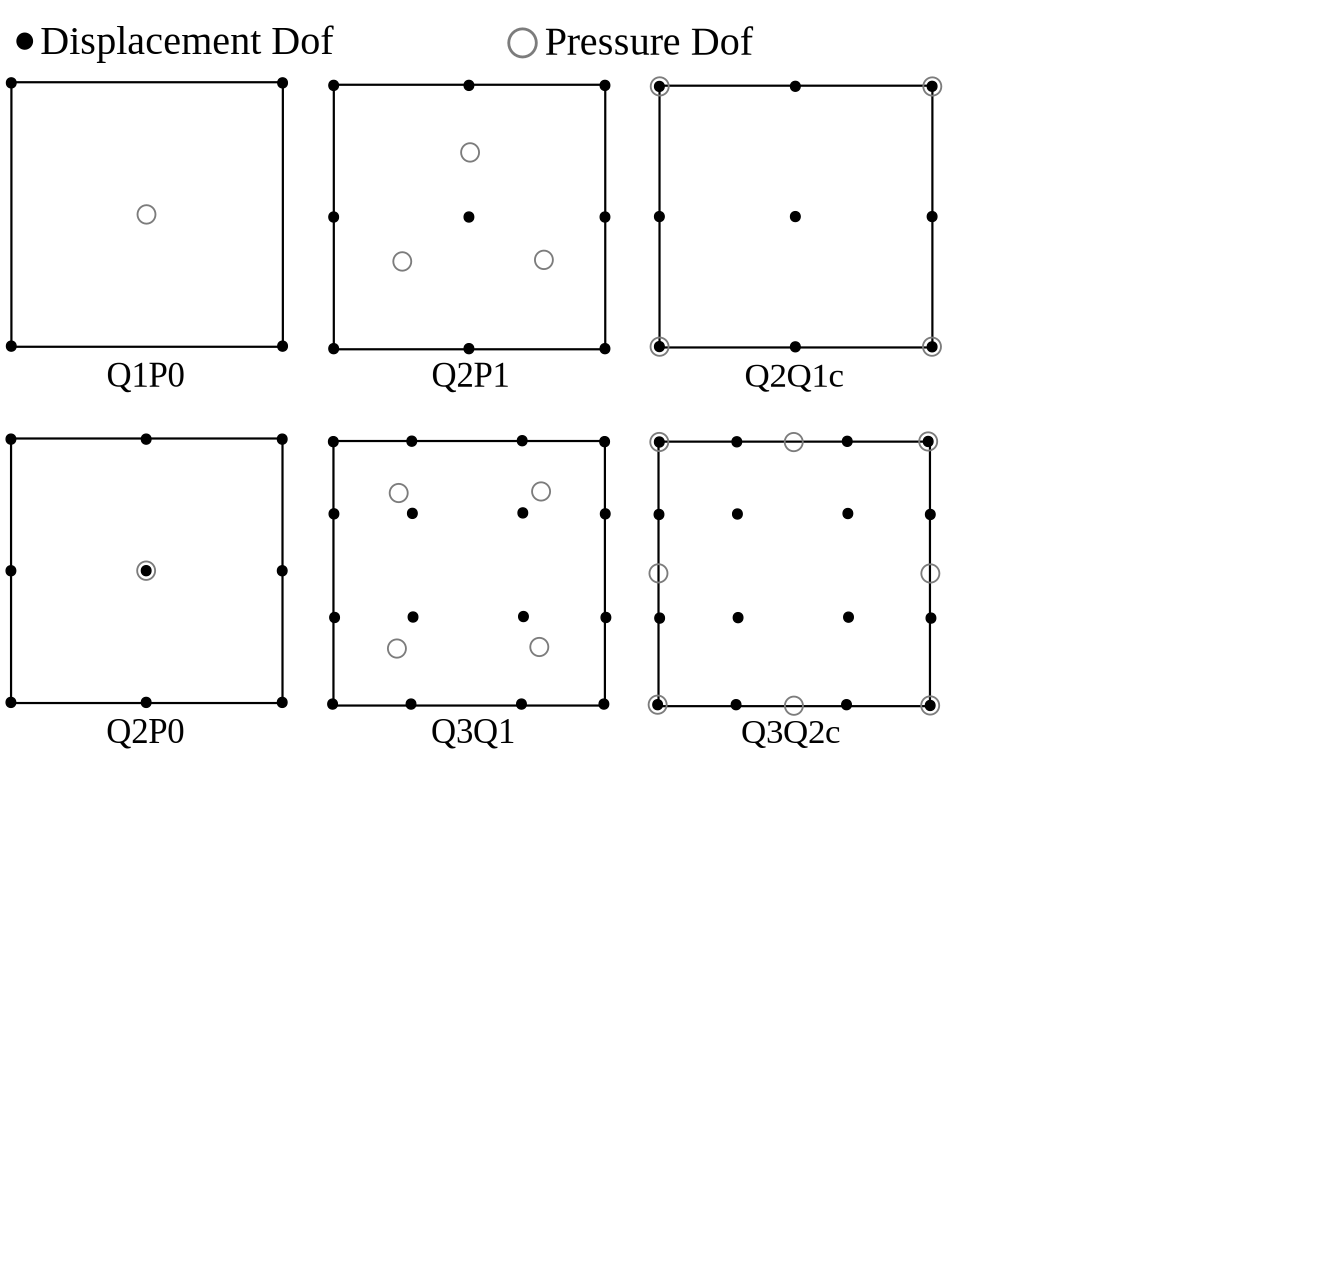
\includegraphics[width=.9\textwidth]{../figs/mixed-element.png}
			\caption{Mixed element with discontinuous and continuous pressure (2D).}
		\end{figure}
	\end{column}
	\end{columns}
\end{frame}

%---------------------------------------------------
\begin{frame}
	\frametitle{Numerical experiment (finite strain, punch test)}
	$E=240.566$ MPa, $(n_x, n_y, n_z) = 2^l (4,4,2)$ with $l \in \{0,1, ..., 4 \}$
	\begin{figure}[H]
		\begin{subfigure}{.5\textwidth}
			\centering
			\includegraphics[width=.8\textwidth]{../figs/Punch.png}
			\caption{Kadapa et al. (2022)}
		\end{subfigure}%
		\begin{subfigure}{.5\textwidth}
			\centering
			\includegraphics[width=.8\textwidth]{../figs/Q2P0-160MPa-dm2.png}
			\caption{}
		\end{subfigure}
		\caption{3D block: (a) geometry and boundary conditions and (b) deformed shape under compression load $p_0=160$ MPa and $\nu=0.49999$ at refinement level $l=2$.}
		\label{fig:block-geometry-boundary}
	\end{figure}
\end{frame}

%---------------------------------------------------
\begin{frame}
	\frametitle{Punch test, displacement convergence study}
	\begin{figure}[H]
		\begin{subfigure}{.5\textwidth}
			\centering
			\includegraphics[width=.8\textwidth]{../figs/u-punch2-iso-0.3.pdf}
			\caption{Single field model $\nu = 0.3$.}
		\end{subfigure}%
		\begin{subfigure}{.5\textwidth}
			\centering
			\includegraphics[width=.8\textwidth]{../figs/u-punch2-iso-0.499.pdf}
			\caption{Single field model $\nu = 0.499$.}
		\end{subfigure}
		\begin{subfigure}{.5\textwidth}
			\centering
			\includegraphics[width=.8\textwidth]{../figs/u-punch2-mixed-0.3.pdf}
			\caption{Mixed fields model $\nu = 0.3$.}
		\end{subfigure}%
		\begin{subfigure}{.5\textwidth}
			\centering
			\includegraphics[width=.8\textwidth]{../figs/u-punch2-mixed-0.49999.pdf}
			\caption{Mixed fields model $\nu = 0.49999$.}
		\end{subfigure}
		%\caption{Displacement results for punch test convergence study for Neo-Hookean model in incompressible regime using single field formulation (top row), non-symmetric mixed formulation (middle row), and perturbed Lagrange-multiplier approach (bottom row).}
	\end{figure}
\end{frame}

%---------------------------------------------------
\begin{frame}
	\frametitle{Punch test, pressure convergence study}
	\begin{figure}[H]
		\begin{subfigure}{.5\textwidth}
			\centering
			\includegraphics[width=.8\textwidth]{../figs/p-punch2-iso-0.3.pdf}
			\caption{Single field model $\nu = 0.3$.}
		\end{subfigure}%
		\begin{subfigure}{.5\textwidth}
			\centering
			\includegraphics[width=.8\textwidth]{../figs/p-punch2-iso-0.499.pdf}
			\caption{Single field model $\nu = 0.499$.}
		\end{subfigure}
		\begin{subfigure}{.5\textwidth}
			\centering
			\includegraphics[width=.8\textwidth]{../figs/p-punch2-mixed-0.3.pdf}
			\caption{Mixed fields model $\nu = 0.3$.}
		\end{subfigure}%
		\begin{subfigure}{.5\textwidth}
			\centering
			\includegraphics[width=.8\textwidth]{../figs/p-punch2-mixed-0.49999.pdf}
			\caption{Mixed fields model $\nu = 0.49999$.}
		\end{subfigure}
		%\caption{Pressure results for punch test convergence study for Neo-Hookean model in incompressible regime using single field formulation (top row), non-symmetric mixed formulation (middle row), and perturbed Lagrange-multiplier approach (bottom row).}
		%\label{fig:punch-pressure-convergence-study-2}
	\end{figure}
\end{frame}

%---------------------------------------------------
\begin{frame}
	\frametitle{Punch test, KSP iteration}
	\begin{figure}[H]
		\begin{subfigure}{.5\textwidth}
			\centering
			\includegraphics[width=.8\textwidth]{../figs/KSPiter-punch2-iso-0.3.pdf}
			\caption{Single field model $\nu = 0.3$.}
		\end{subfigure}%
		\begin{subfigure}{.5\textwidth}
			\centering
			\includegraphics[width=.8\textwidth]{../figs/KSPiter-punch2-iso-0.499.pdf}
			\caption{Single field model $\nu = 0.499$.}
		\end{subfigure}
		\begin{subfigure}{.5\textwidth}
			\centering
			\includegraphics[width=.8\textwidth]{../figs/KSPiter-punch2-mixed-0.3.pdf}
			\caption{Mixed fields model $\nu = 0.3$.}
		\end{subfigure}%
		\begin{subfigure}{.5\textwidth}
			\centering
			\includegraphics[width=.8\textwidth]{../figs/KSPiter-punch2-mixed-0.49999.pdf}
			\caption{Mixed fields model $\nu = 0.49999$.}
		\end{subfigure}
		%\caption{Linear iteration counts for punch test convergence study for Neo-Hookean model in incompressible regime using single field formulation (top row), non-symmetric mixed formulation (middle row), and perturbed Lagrange-multiplier approach (bottom row).}
		%\label{fig:punch-iter-study-2}
	\end{figure}
\end{frame}

%---------------------------------------------------
\begin{frame}
	\frametitle{Punch test, displacement and pressure distribution}
	\begin{figure}[H]
		\begin{subfigure}{.5\textwidth}
			\centering
			\includegraphics[width=.68\textwidth]{../figs/u-Q3-320MPa-0.3.png}
			\caption{Displacement $Q_3$.}
		\end{subfigure}%
		\begin{subfigure}{.5\textwidth}
			\centering
			\includegraphics[width=.68\textwidth]{../figs/p-Q3-320MPa-0.3.png}
			\caption{Pressure $Q_3$.}
		\end{subfigure}
		\begin{subfigure}{.5\textwidth}
			\centering
			\includegraphics[width=.68\textwidth]{../figs/u-Q3Q2-320MPa-0.3.png}
			\caption{Displacement $Q_3Q_2$.}
		\end{subfigure}%
		\begin{subfigure}{.5\textwidth}
			\centering
			\includegraphics[width=.68\textwidth]{../figs/p-Q3Q2-320MPa-0.3.png}
			\caption{Pressure $Q_3Q_2$.}
		\end{subfigure}
		\caption*{$p_0=320$ MPa with mesh refinement level $l=3$, and \alert{$\nu = 0.3$}.}
		%\label{fig:punch2-rel-error-u}
	\end{figure}
\end{frame}

%---------------------------------------------------
\begin{frame}
	\frametitle{Punch test, displacement and pressure distribution}
	\begin{figure}[H]
		\begin{subfigure}{.5\textwidth}
			\centering
			\includegraphics[width=.68\textwidth]{../figs/u-Q3-320MPa-0.495.png}
			\caption{Displacement $Q_3$.}
		\end{subfigure}%
		\begin{subfigure}{.5\textwidth}
			\centering
			\includegraphics[width=.68\textwidth]{../figs/p-Q3-320MPa-0.495.png}
			\caption{Pressure $Q_3$.}
		\end{subfigure}
		\begin{subfigure}{.5\textwidth}
			\centering
			\includegraphics[width=.68\textwidth]{../figs/u-Q3Q2-320MPa-0.495.png}
			\caption{Displacement $Q_3Q_2$.}
		\end{subfigure}%
		\begin{subfigure}{.5\textwidth}
			\centering
			\includegraphics[width=.68\textwidth]{../figs/p-Q3Q2-320MPa-0.495.png}
			\caption{Pressure $Q_3Q_2$.}
		\end{subfigure}
		\caption*{$p_0=320$ MPa with mesh refinement level $l=3$, and \alert{$\nu = 0.495$}.}
		%\label{fig:punch2-rel-error-u}
	\end{figure}

\end{frame}

%---------------------------------------------------
\begin{frame}
	\frametitle{Computation cost of $\bm u$-based vs $\bm u -p$ formulations}
	\onslide<1->{\begin{table}[H]
		%\caption{Total DoFs, SNES iteration at each pseudo time step, KSP iteration per Newton solver step, condition number of the preconditioned operator, and solve time for the block under compression in compressible and incompressible limits.}
		\centering
		\begin{tabular}{l*{5}{c}}
		\toprule
		\multicolumn{1}{c}{}  & \multicolumn{4}{c}{$Q_3$, Total DoFs: 1.35 MDoFs} \\
		\cmidrule(r){2-5}
		\multicolumn{1}{c}{$\nu$} & \multicolumn{1}{c}{SNES Its} & \multicolumn{1}{c}{KSP Its} & \multicolumn{1}{c}{Condition number} & \multicolumn{1}{c}{Solve time (sec)} \\
		\midrule
		0.3   & 5 & 7  & 3  & 175.253 \\
		0.495 & 7 & 30 & 67 & \alert{689.826} \\
		\bottomrule
		\end{tabular}
	\end{table}}
	\onslide<2->{\begin{table}[H]
		%\caption{Total DoFs, SNES iteration at each pseudo time step, KSP iteration per Newton solver step, condition number of the preconditioned operator, and solve time for the block under compression in compressible and incompressible limits.}
		\centering
		\begin{tabular}{l*{5}{c}}
		\toprule
		\multicolumn{1}{c}{}  & \multicolumn{4}{c}{$Q_3Q_2$, Total DoFs: 1.48 MDoFs} \\
		\cmidrule(r){2-5}
		\multicolumn{1}{c}{$\nu$} & \multicolumn{1}{c}{SNES Its} & \multicolumn{1}{c}{KSP Its} & \multicolumn{1}{c}{Condition number} & \multicolumn{1}{c}{Solve time (sec)} \\
		\midrule
		0.3   & 5  & 8  & 9 &  208.126 \\
		0.495 & 5  & 13 & 3 &  \alert{289.666} \\
		\bottomrule
		\end{tabular}
	\end{table}}
	\onslide<3->{\begin{tcolorbox}
		Even if we only need displacement results, it is \alert{cheaper} to run mixed formulation when $\nu \to 0.5$.
	\end{tcolorbox}}
\end{frame}

%---------------------------------------------------
\begin{frame}
	\frametitle{Efficiency of the Sparse direct solver vs Matrix-free}
	\begin{figure}[h]
		\center\includegraphics[width=.8\textwidth]{../figs/efficiency-chol-chol.pdf}
		\caption*{Sparse matrix, Cholesky-Cholesky.}
	\end{figure}	
	\alert{Approximating $\mathcal{\hat A}^{-1}, \mathcal{\hat D}^{-1}$ by Cholesky factorization.}
\end{frame}

%---------------------------------------------------
\begin{frame}
	\frametitle{Efficiency of the Sparse matrix vs Matrix-free}
	\begin{figure}[H]
		\begin{subfigure}{.5\textwidth}
			\centering
			\includegraphics[width=.8\textwidth]{../figs/efficiency-chol-chol.pdf}
			\caption{Sparse matrix, Cholesky-Cholesky.}
		\end{subfigure}%
		\begin{subfigure}{.5\textwidth}
			\centering
			\includegraphics[width=.8\textwidth]{../figs/efficiency-amg-amg.pdf}
			\caption{Sparse matrix, AMG-AMG.}
		\end{subfigure}
		\begin{subfigure}{.5\textwidth}
			\centering
			\includegraphics[width=.8\textwidth]{../figs/efficiency-amg-jac.pdf}
			\caption{Sparse matrix, AMG-Jacobi.}
		\end{subfigure}%
		\begin{subfigure}{.5\textwidth}
			\centering
			\includegraphics[width=.8\textwidth]{../figs/efficiency-pmg-jac.pdf}
			\caption{Matrix-free, pMG-Jacobi.}
		\end{subfigure}
	\end{figure}	
\end{frame}

%---------------------------------------------------
\begin{frame}
	\frametitle{Element aspect ratio effect on efficiency/robustness}
	\begin{figure}[H]
		\begin{subfigure}{.5\textwidth}
			\centering
			\includegraphics[width=.8\textwidth]{../figs/von-mises-schwarz1.png}
			%\caption{thickness 0.2 }
		\end{subfigure}%
		\begin{subfigure}{.5\textwidth}
			\centering
			\includegraphics[width=.8\textwidth]{../figs/von-mises-schwarz2.png}
			%\caption{thickness 0.1 }
		\end{subfigure}
		\caption{Displacement distribution for schwarz mesh with refinement level $l=2$, 2 layers, and extent (2,2,2) using mixed Neo-Hookean model (left) thickness 0.2 under 4 Mpa compression, (right) thickness 0.1 under 2.35 Mpa compression.}
		%\label{fig:schwarz-deformed}
	\end{figure}
\end{frame}

%---------------------------------------------------
\begin{frame}
	\frametitle{Schwarz thickness 0.2, displacement convergence study}
	\begin{figure}[H]
		\begin{subfigure}{.5\textwidth}
			\centering
			\includegraphics[width=.8\textwidth]{../figs/u-schwarz1-mixed-0.3.pdf}
			\caption{Mixed model $\nu = 0.3$.}
		\end{subfigure}%
		\begin{subfigure}{.5\textwidth}
			\centering
			\includegraphics[width=.8\textwidth]{../figs/u-schwarz1-mixed-0.498.pdf}
			\caption{Mixed model $\nu = 0.498$.}
		\end{subfigure}
		%\caption{Displacement convergence study result for schwarz mesh with thickness 0.2 under 4 MPa compressible load with Neo-Hookean model in compressible and incompressible regimes using non-symmetric mixed formulation (top row), and perturbed Lagrange-multiplier approach (bottom row).}
		%\label{fig:schwarz-disp-convergence-study-1}
	\end{figure}
\end{frame}

%---------------------------------------------------
\begin{frame}
	\frametitle{Schwarz thickness 0.2, KSP iteration}
	\begin{figure}[H]
		\begin{subfigure}{.5\textwidth}
			\centering
			\includegraphics[width=.8\textwidth]{../figs/KSPiter-schwarz1-mixed-0.3.pdf}
			\caption{Mixed model $\nu = 0.3$.}
		\end{subfigure}%
		\begin{subfigure}{.5\textwidth}
			\centering
			\includegraphics[width=.8\textwidth]{../figs/KSPiter-schwarz1-mixed-0.498.pdf}
			\caption{Mixed model $\nu = 0.498$.}
		\end{subfigure}
		%\caption{Linear iteration count for schwarz mesh with thickness 0.2 under 4 MPa compressible load with Neo-Hookean model in compressible and incompressible regimes using non-symmetric mixed formulation (top row), and perturbed Lagrange-multiplier approach (bottom row).}
		%\label{fig:schwarz-iter-study-1}
	\end{figure}
\end{frame}

%---------------------------------------------------
\begin{frame}
	\frametitle{Schwarz thickness 0.1, displacement convergence study}
	\begin{figure}[H]
		\begin{subfigure}{.5\textwidth}
			\centering
			\includegraphics[width=.8\textwidth]{../figs/u-schwarz2-mixed-0.3.pdf}
			\caption{Mixed model $\nu = 0.3$.}
		\end{subfigure}%
		\begin{subfigure}{.5\textwidth}
			\centering
			\includegraphics[width=.8\textwidth]{../figs/u-schwarz2-mixed-0.498.pdf}
			\caption{Mixed model $\nu = 0.498$.}
		\end{subfigure}
		%\caption{Displacement convergence study result for schwarz mesh with thickness 0.2 under 4 MPa compressible load with Neo-Hookean model in compressible and incompressible regimes using non-symmetric mixed formulation (top row), and perturbed Lagrange-multiplier approach (bottom row).}
		%\label{fig:schwarz-disp-convergence-study-1}
	\end{figure}
\end{frame}

%---------------------------------------------------
\begin{frame}
	\frametitle{Schwarz thickness 0.1, KSP iteration}
	\begin{figure}[H]
		\begin{subfigure}{.5\textwidth}
			\centering
			\includegraphics[width=.8\textwidth]{../figs/KSPiter-schwarz2-mixed-0.3.pdf}
			\caption{Mixed model $\nu = 0.3$.}
		\end{subfigure}%
		\begin{subfigure}{.5\textwidth}
			\centering
			\includegraphics[width=.8\textwidth]{../figs/KSPiter-schwarz2-mixed-0.498.pdf}
			\caption{Mixed model $\nu = 0.498$.}
		\end{subfigure}
		%\caption{Linear iteration count for schwarz mesh with thickness 0.2 under 4 MPa compressible load with Neo-Hookean model in compressible and incompressible regimes using non-symmetric mixed formulation (top row), and perturbed Lagrange-multiplier approach (bottom row).}
		%\label{fig:schwarz-iter-study-1}
	\end{figure}
\end{frame}

%---------------------------------------------------
\begin{frame}
	\frametitle{Conclusion and future work}
	\begin{columns}
		\begin{column}{0.5\textwidth}<1->
			\begin{figure}
				\center\includegraphics[angle=0,width=0.9\textwidth]{../figs/summary.png}
			\end{figure}
		\end{column}
		\begin{column}{0.5\textwidth}
			\begin{itemize}
				\item<2-> \small{When $\nu \to 0.5$, $\bm u$-based formulation shows fluctuation in pressure response even with high-order element but almost accurate results in displacement.}
				\item<3-> \small{Solve time of $\bm u - p$ simulation is less than single field case when $\nu \to 0.5$.}
				\item<4-> \small{KSP iteration count, and largest eigenvalue are smaller for $\nu_p > 0$}
			\end{itemize}
		\end{column}
	\end{columns}

	\small{
	\begin{itemize}
		\item<5-> Stable constitutive formulation opens a door for hyperelastic simulation using single or mixed precision.
		\item<6-> With this implemented mixed formulation in Ratel, we can simulate all other mixed problems like poroelasticity, phase field modeling, ...
	\end{itemize}}
\end{frame}

%---------------------------------------------------
\begin{frame}{More GPU results and stable constitutive formulation}
	\textit{Crusher, \, Summit, \, Lassen, \, Perlmutter}
	\begin{figure} [h]
		\includegraphics[width=0.8\textwidth]{../figs/paper.png}
	\end{figure}

	\vspace{10mm}
	\textbf{Stable numerics for finite-strain elasticity}
	
	Rezgar Shakeri, Leila Ghaffari, Jeremy L. Thompson, Jed Brown
\end{frame}

%==================================================
% Back-up slides
%==================================================

\begin{frame}
	\huge Back-up slides
\end{frame}

%---------------------------------------------------
\begin{frame}
	\frametitle{Stable constitutive modeling}
	
	\begin{itemize}
		\item<1-> $\emachine = \sup_{x} \lvert \fl(x) - x \rvert / \lvert x \rvert$.
		\item<1-> Elementary math operators \alert{$\circledast$} (standing for addition, subtraction, multiplication, or division)
		
		\vspace{5mm}
		$x \circledast y = \fl(x \ast y)$, \quad $\lvert x \circledast y - x \ast y\rvert / \lvert x \ast y \rvert \le \emachine$
		
		\vspace{10mm}
		\item<2-> How about $(x \circledast y) \circledast z$ ?
		
		\vspace{5mm}
		$(x \oplus 1) \ominus 1 = 0$ for $x=10^{-16}$ has a \alert{relative error of $1$.}
	\end{itemize}
	
	
	\begin{block}{Remark}<1>
		Machine epsilon or machine precision is an upper bound on the relative approximation error due to rounding in floating point arithmetic. \alert{$\emachine \approx 10^{-16}$} for double precision and \alert{$6 \times 10^{-8}$} for single precision.
	\end{block}
\end{frame}

%---------------------------------------------------
\begin{frame}
	\frametitle{Stable constitutive modeling}
	\begin{figure} [h]
		\includegraphics[width=\textwidth]{../figs/rounding-cond.pdf}
		%\caption{The stair-step patterns illustrate numerical instability evaluating in $(1 + x)-1$ (left) and $\log(1+x)$ (center). When evaluating $(1 + x) - 1$, a small relative error is incurred in the well-conditioned operation $s := 1 + x$, and that error becomes a large relative error because $s - 1$ has unbounded condition number as $s\to 1$ (right), despite this operation being computed exactly in floating point arithmetic.}
	\end{figure}
	$s := 1 + x$, $f(s) = s - 1$ has unbounded condition number as $s\to 1$ (right), despite this operation being computed exactly in floating point arithmetic.
\end{frame}

%---------------------------------------------------
\begin{frame}
	\frametitle{Stable constitutive modeling}
	\textbf{Stable computation of strain}
	
	\vspace{10mm}
	\begin{equation}
		\boldsymbol{E} =  \frac{1}{2} \left(\boldsymbol C - \boldsymbol{I} \right) = \frac{1}{2} \left(\boldsymbol{F}^T \boldsymbol{F} - \boldsymbol{I} \right) \nonumber
	\end{equation}
	We substitute $\boldsymbol F = \boldsymbol I + \boldsymbol H$, where $\boldsymbol H = \nabla_X \boldsymbol u$
	
	\begin{equation}
		\boldsymbol{E} =  \frac{1}{2} \left(\boldsymbol H + \boldsymbol H^T + \boldsymbol H^T \boldsymbol H \right) \nonumber
	\end{equation}
\end{frame}

%---------------------------------------------------
\begin{frame}
	\frametitle{Stable constitutive modeling}
	\textbf{Stable computation of $J=\Det{\bm F}$}
	
	\vspace{10mm}
	Consider the 2-dimensional case
	$$
	\bm F = \bm I + \bm H = \bm I + \nabla_X \bm{u} = \begin{bmatrix}
		1 + u_{1,1} & u_{1,2} \\
		u_{2,1} & 1 + u_{2,2}
	\end{bmatrix},
	$$
	and let compute $\Jm = J-1$ by
	\begin{equation}\label{eq:Jm1}
		\Jm = u_{1,1} + u_{2,2} + u_{1,1} u_{2,2} - u_{1,2} u_{2,1}. \nonumber
	\end{equation}
	then $J = \Jm + 1$.
\end{frame}

%---------------------------------------------------
\begin{frame}
	\frametitle{Stable constitutive modeling}
	\begin{figure}
		\centering
		\includegraphics[width=.6\linewidth]{../figs/Jm1.pdf}
		\caption{Relative error of standard computation of $J-1$ and its stable way $\Jm$} \label{fig1:Jm1}
	\end{figure}
	
	%\vspace{15mm}
	\begin{block}{Remark}
		The standard computation for a strain of order \alert{$10^{-m}$} will result in \alert{$m$} digits lost in the computed stress.
	\end{block}
\end{frame}

%---------------------------------------------------
\begin{frame}
	\frametitle{Stable constitutive modeling}
	\begin{figure} [h]
		\includegraphics[width=\textwidth]{../figs/table-constitutive.png}
		%\caption{The stair-step patterns illustrate numerical instability evaluating in $(1 + x)-1$ (left) and $\log(1+x)$ (center). When evaluating $(1 + x) - 1$, a small relative error is incurred in the well-conditioned operation $s := 1 + x$, and that error becomes a large relative error because $s - 1$ has unbounded condition number as $s\to 1$ (right), despite this operation being computed exactly in floating point arithmetic.}
	\end{figure}
	
	\vspace{10mm}
	{We have implemented, \alert{Neo-Hookean, Mooney-Rivlin}, and \alert{Ogden} in a stable way in Ratel.}
\end{frame}

%---------------------------------------------------
\begin{frame}
	\frametitle{Inf-sup stability}

	Find $\lambda \in \mathbb{R}$, $0 \neq (\boldsymbol u_h, p_h) \in \mathbb{V}_h \times \mathbb{Q}_h $, such that for all $(\boldsymbol v, q) \in \mathbb{V}_h^0 \times \mathbb{Q}_h$

	\begin{equation*}
		a(\boldsymbol v, \boldsymbol u) + b(\boldsymbol v, p) + b(q, \boldsymbol u) = -\lambda \langle p, q \rangle_{\mathbb{Q}} 
	\end{equation*}
	
	then, $\lambda \geq 0$ and inf-sup constant is $\beta = \sqrt{\lambda_{\text{min}}}$, $\quad \beta \geq \beta_h >0$ 

	\vspace{5mm}
	\begin{figure}[h]
		\center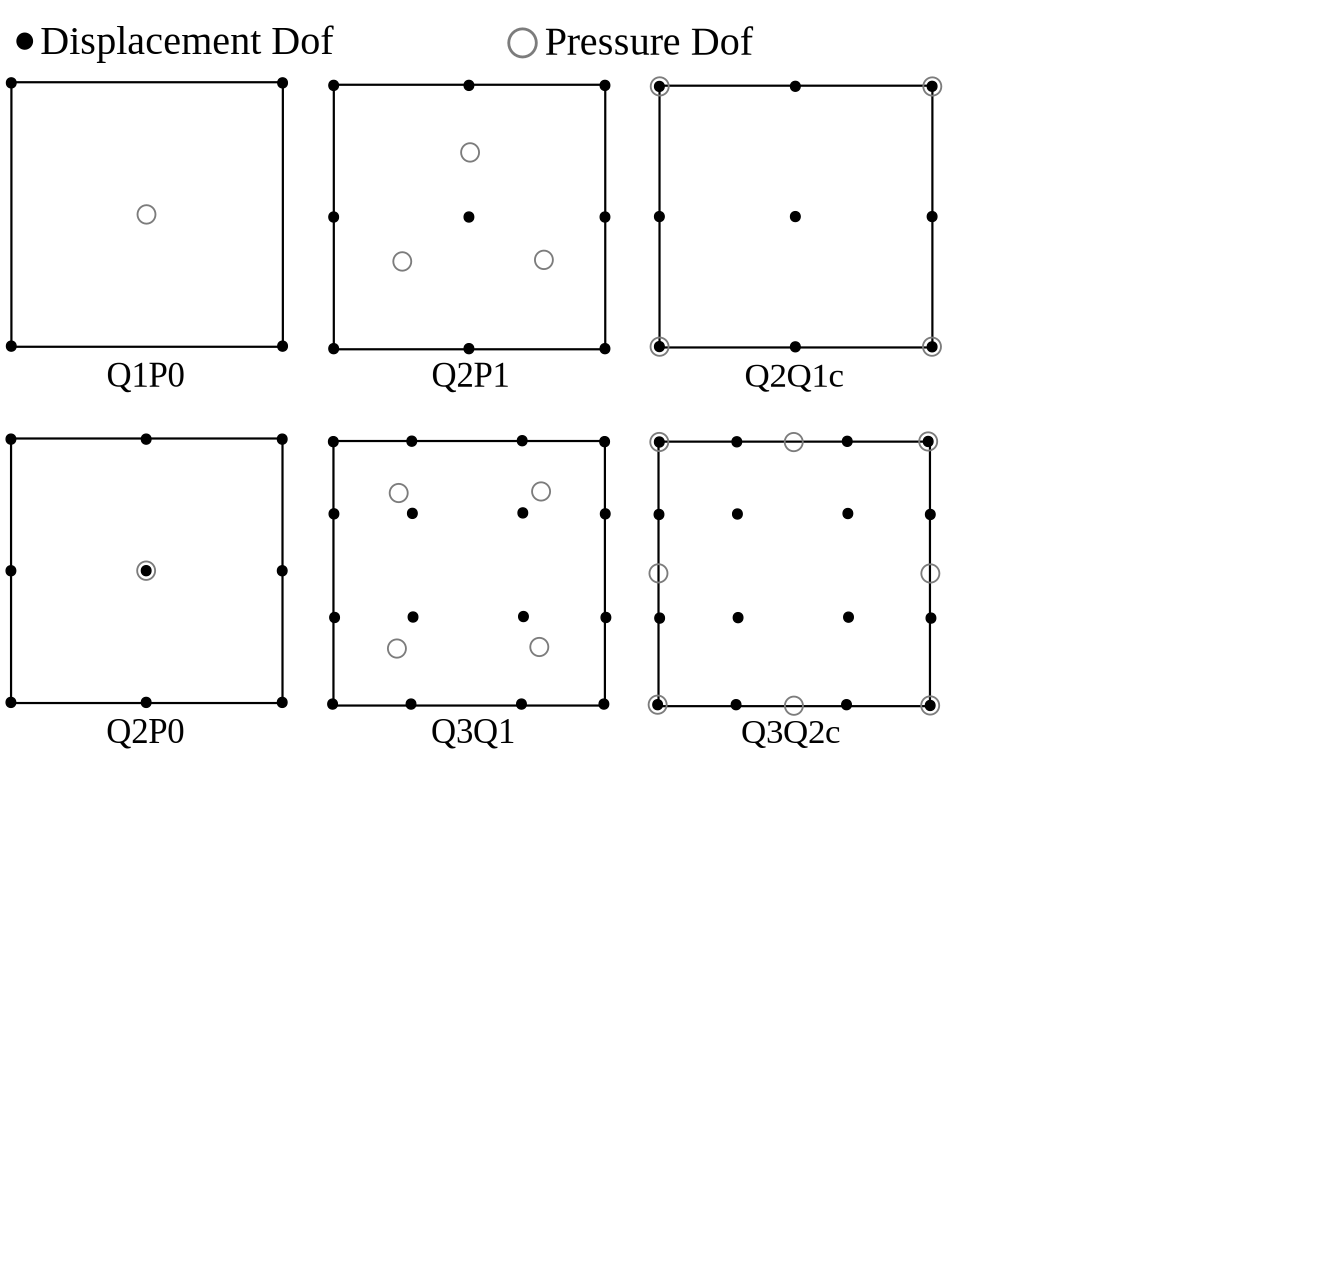
\includegraphics[width=.4\textwidth]{../figs/mixed-element.png}
		\caption{Mixed element with discontinuous and continuous pressure (2D).}
	\end{figure}
\end{frame}

%---------------------------------------------------
\begin{frame}
	\frametitle{Inf-sup stability- continuous pressure}

	\begin{figure} [H]
		\begin{subfigure}{.5\textwidth}
			\centering
			\includegraphics[width=.9\textwidth]{../figs/cont-p-1.png}
		\end{subfigure}%
		\begin{subfigure}{.5\textwidth}
			\centering
			\includegraphics[width=.9\textwidth]{../figs/cont-p-10.png}
		\end{subfigure}
		%\caption{Inf-sup constant for various mixed-elements with continuous (top row) and discontinuous (bottom row) pressure on square and stretched meshes.}
		%\label{fig:inf-sup}
	\end{figure}
\end{frame}

%---------------------------------------------------
\begin{frame}
	\frametitle{Inf-sup stability- discontinuous pressure}

	\begin{figure} [H]
		\begin{subfigure}{.5\textwidth}
			\centering
			\includegraphics[width=.9\textwidth]{../figs/dist-p-1.png}
		\end{subfigure}%
		\begin{subfigure}{.5\textwidth}
			\centering
			\includegraphics[width=.9\textwidth]{../figs/dist-p-10.png}
		\end{subfigure}
		%\caption{Inf-sup constant for various mixed-elements with continuous (top row) and discontinuous (bottom row) pressure on square and stretched meshes.}
		%\label{fig:inf-sup}
	\end{figure}
\end{frame}

%---------------------------------------------------
\begin{frame}
	\frametitle{Convergence study- continuous pressure}

	\begin{figure} [h]
		\includegraphics[width=0.8\textwidth]{../figs/convergence-order-cont.png}
	\end{figure}

\end{frame}

%---------------------------------------------------
\begin{frame}
	\frametitle{Convergence study- discontinuous pressure}

	\begin{figure} [h]
		\includegraphics[width=0.8\textwidth]{../figs/convergence-order-disc.png}
	\end{figure}

\end{frame}

%---------------------------------------------------
\begin{frame}
	\frametitle{Punch test, displacement and pressure distribution}
	\begin{figure}[H]
		\begin{subfigure}{.5\textwidth}
			\centering
			\includegraphics[width=.68\textwidth]{../figs/u-Q3Q2-320MPa-0.5.png}
			\caption{Displacement $Q_3Q_2$.}
		\end{subfigure}%
		\begin{subfigure}{.5\textwidth}
			\centering
			\includegraphics[width=.68\textwidth]{../figs/p-Q3Q2-320MPa-0.5.png}
			\caption{Pressure $Q_3Q_2$.}
		\end{subfigure}
		\begin{subfigure}{.5\textwidth}
			\centering
			\includegraphics[width=.68\textwidth]{../figs/J-Q3Q2-320MPa-0.495.png}
			\caption{J, $Q_3Q_2$, $\nu=0.495$.}
		\end{subfigure}%
		\begin{subfigure}{.5\textwidth}
			\centering
			\includegraphics[width=.68\textwidth]{../figs/J-Q3Q2-320MPa-0.5.png}
			\caption{J, $Q_3Q_2$, $\nu=0.5$.}
		\end{subfigure}
		\caption*{$p_0=320$ MPa with mesh refinement level $l=3$, and Poisson's ratio 0.5.}
		%\label{fig:punch2-rel-error-u}
	\end{figure}
	
\end{frame}
%---------------------------------------------------

\begin{frame}
		\frametitle{See $\nu = 0.5$ results}
		\begin{table}[H]
		%\caption{Total DoFs, SNES iteration at each pseudo time step, KSP iteration per Newton solver step, condition number of the preconditioned operator, and solve time for the block under compression in compressible and incompressible limits.}
		\centering
		\begin{tabular}{l*{5}{c}}
			\toprule
			\multicolumn{1}{c}{}  & \multicolumn{4}{c}{$Q_3$, Total DoFs: 1345584} \\
			\cmidrule(r){2-5}
			\multicolumn{1}{c}{$\nu$} & \multicolumn{1}{c}{SNES Its} & \multicolumn{1}{c}{KSP Its} & \multicolumn{1}{c}{Condition number} & \multicolumn{1}{c}{Solve time (sec)} \\
			\midrule
			0.3   & 5 & 7  & 3  & 175.253 \\
			0.495 & 7 & 30 & 67 & \alert{689.826} \\
			\midrule
			\multicolumn{1}{c}{}  & \multicolumn{4}{c}{$Q_3Q_2$, Total DoFs: 1485009} \\
			\cmidrule(r){2-5}
			\multicolumn{1}{c}{$\nu$} & \multicolumn{1}{c}{SNES Its} & \multicolumn{1}{c}{KSP Its} & \multicolumn{1}{c}{Condition number} & \multicolumn{1}{c}{Solve time (sec)} \\
			\midrule
			0.3   & 5  & 8  & 9 &  208.126 \\
			0.495 & 5  & 13 & 3 &  \alert{289.666} \\
			0.5   & 5  & 13 & 3 &  933.915  \\
			\bottomrule
		\end{tabular}
	\end{table}

Only solve time is different
\end{frame}

\end{document} 